% ------------------------------------------------------------------------------
% TYPO3 Version 10.1 - What's New (German Version)
%
% @license	Creative Commons BY-NC-SA 3.0
% @link		http://typo3.org/download/release-notes/whats-new/
% @language	German
% ------------------------------------------------------------------------------

\section{Backend User Interface}
\begin{frame}[fragile]
	\frametitle{Backend User Interface}

	\begin{center}\huge{Kapitel 1:}\end{center}
	\begin{center}\huge{\color{typo3darkgrey}\textbf{Backend User Interface}}\end{center}

\end{frame}

% ------------------------------------------------------------------------------
% Feature | 89115 | Auto slug update and redirect creation on slug change

\begin{frame}[fragile]
	\frametitle{Backend User Interface}
	\framesubtitle{Slug-Updates und Weiterleitungen (1)}

	\begin{itemize}
		\item Wenn Backend-Benutzer den URL-Pfad einer Seite ändern (den sogenannten "Slug"),
			wird die alte URL nicht mehr verfügbar.
		\item Dies führt möglicherweise zu einem "Seite nicht gefunden" Fehler, 
			auch für die URLs aller Unterseiten.
	\end{itemize}

	\begin{figure}
		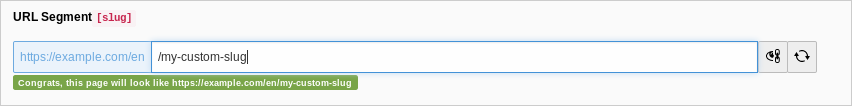
\includegraphics[width=0.80\linewidth]{BackendUserInterface/89115b-AutoSlugUpdateAndRedirectCreationOnSlugChange.png}
	\end{figure}

	\begin{itemize}
		\item Im Rahmen der TYPO3 Version 10.1, wird dies durch zwei Aktionen verhindert:

			\begin{itemize}
				\item Slugs werden für alle Unterseiten  automatisch aktualisiert
				\item Es werden Weiterleitungen von den alten zu den neuen URLs erstellt
			\end{itemize}

	\end{itemize}

\end{frame}

% ------------------------------------------------------------------------------
% Feature | 89115 | Auto slug update and redirect creation on slug change

\begin{frame}[fragile]
	\frametitle{Backend User Interface}
	\framesubtitle{Slug-Updates und Weiterleitungen (2)}

	\begin{itemize}
		\item Backend-Benutzer werden über diese Aktionen informiert und können
			die Änderungen bei Bedarf einfach per Mausklick rückgängig machen:

	\end{itemize}

	\begin{figure}
		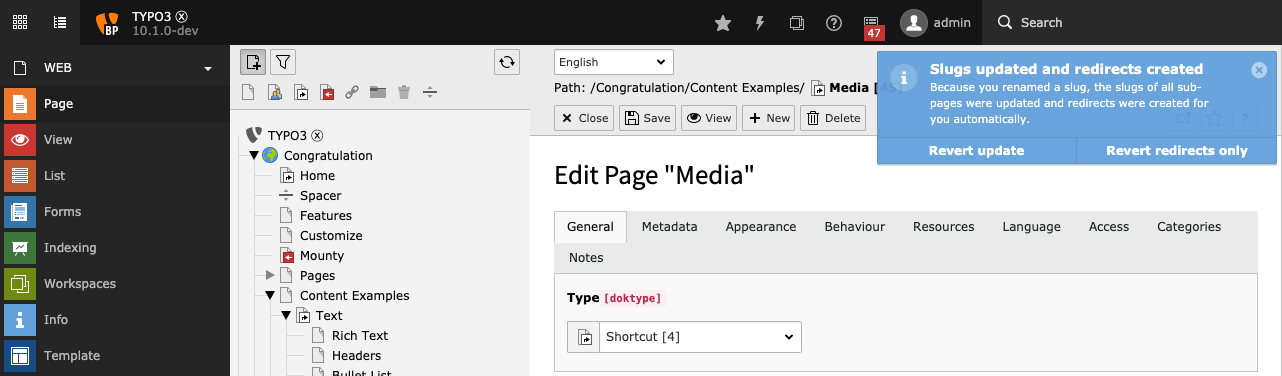
\includegraphics[width=0.80\linewidth]{BackendUserInterface/89115c-AutoSlugUpdateAndRedirectCreationOnSlugChange.png}
	\end{figure}

\end{frame}

% ------------------------------------------------------------------------------
% Feature | 85918 | Hide in menu / Show in menu entry for pages in context menu

\begin{frame}[fragile]
	\frametitle{Backend User Interface}
	\framesubtitle{Im Menü ein-/ausblenden}

	Ein neuer Eintrag wurde zum Kontextmenü hinzugefügt, um Seiten im Menü anzuzeigen/auszublenden.

	\begin{figure}
		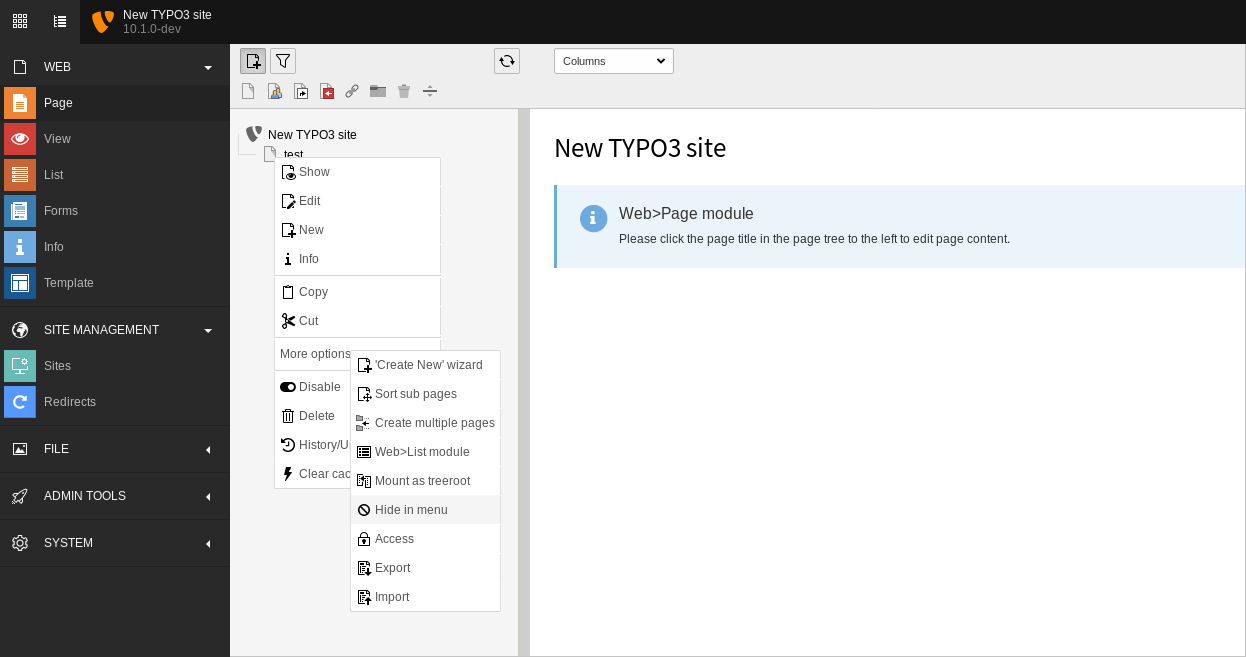
\includegraphics[width=0.80\linewidth]{BackendUserInterface/85918-HideShowInMenu-InContextMenu.png}
	\end{figure}

\end{frame}

% ------------------------------------------------------------------------------
